% sample-size.tex


% from http://www.texample.net/tikz/examples/consort-flowchart/
% A CONSORT-style flowchart of a randomized controlled trial
% using the PGF/TikZ package
% Author  : Morten Vejs Willert (July 2010)
% License : Creative Commons attribution license
\documentclass[14pt]{article}
\usepackage[latin1]{inputenc}
\usepackage{lscape}
\usepackage[legalpaper, margin=0.5in]{geometry}
\usepackage{tikz}
\usetikzlibrary{arrows,positioning,arrows.meta,positioning,decorations.markings,shapes, automata, calc, fit,decorations.markings,shapes.geometric,backgrounds}
\tikzset{
  font={\fontsize{12pt}{14}\selectfont}}

%%%<
\usepackage{verbatim}
%\usepackage[active,tightpage]{preview}
%\PreviewEnvironment{center}
%\setlength\PreviewBorder{10pt}%
%%%>
\begin{comment}
:Title: A CONSORT-style flowchart of a randomized controlled trial
:Tags: Matrices, Charts
:Author: Morten Vejs Willert
:Slug: consort-flowchart

A flowchart is an efficient graphical tool for depicting the 
progress of subjects through the phases of a clinical trial. 
This example shows how to use the PGF/TikZ package within a 
LaTeX article class document to make a flowchart of participants
progress through the phases of a randomized controlled trial. 
The flowchart is meant to conform to the specifications of the 
CONSORT 2010 Statement guidelines adhered to by the majority 
of scientific biomedical journals. The author takes no 
responsibility whether this goal has been achieved successfully,
should anyone care to use the example as a template when 
submitting a manuscript of their own to a biomedical journal. 

The basic code regarding placement of the nodes within a matrix, 
as well as for drawing paths between nodes, was adapted from the 
example by Kjell Magne Fauske in 'The TikZ and PGF Packages Manual 
for version 2.00' by Till Tantau.

In the example the tikzpicture-environment is used within a center
environment and \captionof from the caption package, because floating
is not required and conflicts with the preview package. In a common
document, a standard figure environment is recommended, which allows
the addition of a caption to  accompany the flowchart, as well as
options for placement of the float when typesetting the document.
\end{comment}

\usetikzlibrary{shapes,arrows}
\usepackage{caption}
\newcommand*{\h}{\hspace{5pt}}% for indentation
\newcommand*{\hh}{\h\h}% double indentation

\begin{document}
%  \captionof{figure}{Flowchart of participants' progress through
 %  the phases of the study}
  % setting the typeface to sans serif and the font size to small
  % the scope local to the environment
  \sffamily
  \footnotesize
  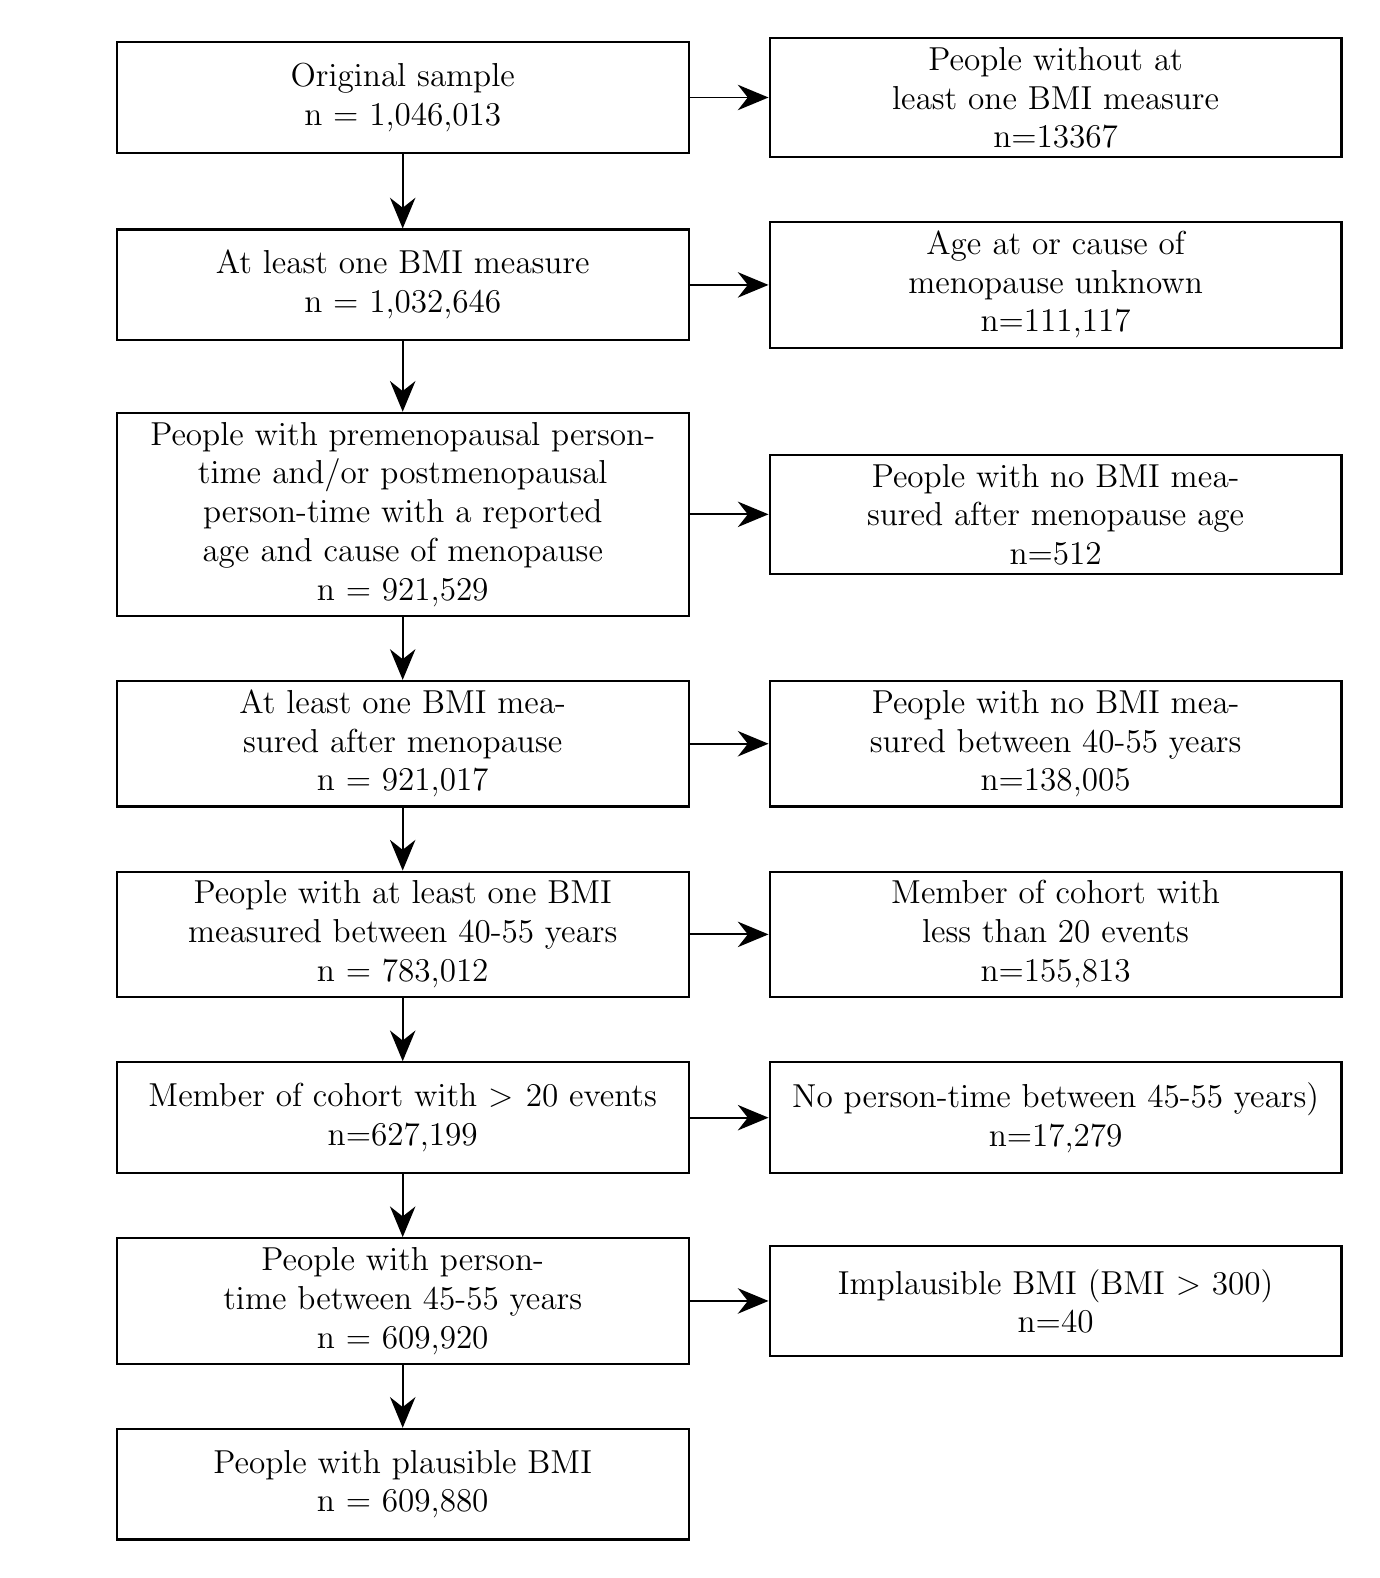
\begin{tikzpicture}[auto,
    %decision/.style={diamond, draw=black, thick, fill=white,
    %text width=8em, text badly centered,
    %inner sep=1pt, font=\sffamily\small},
    block_centerr/.style ={rectangle, draw=black, thick, fill=white,
      text width=20em, text centered, minimum height=4em},
    block_centerrr/.style ={rectangle, draw=black, thick, fill=white,
      text width=30em, text centered, minimum height=4em},
    block_center/.style ={rectangle, draw=black, thick, fill=white,
      text width=12em, text centered, minimum height=4em},
    block_center2/.style ={rectangle, draw=black, thick, fill=white,
      text centered, minimum height=4em},			
    block_clear/.style ={rectangle, draw=none, thick, fill=white,
      text width=12em, text centered, minimum height=4em},
    block_left/.style ={rectangle, draw=black, thick, fill=white,
      text width=16em, text ragged, minimum height=4em, inner sep=6pt},
    block_noborder/.style ={rectangle, draw=none, thick, fill=none,
      text width=18em, text centered, minimum height=1em},
    block_assign/.style ={rectangle, draw=black, thick, fill=white,
      text width=18em, text ragged, minimum height=3em, inner sep=6pt},
    block_lost/.style ={rectangle, draw=black, thick, fill=white,
      text width=16em, text ragged, minimum height=3em, inner sep=6pt},
      line/.style ={draw, ultra thick, -latex', shorten >=0pt},
	paths/.style={draw, ->, ultra thick, >=stealth'},
	paths2/.style={black, draw,
          , line width=0.25mm, arrows={-Stealth[angle=45:12pt, scale=1, black, fill=black]}}]
    % outlining the flowchart using the PGF/TikZ matrix funtion
    \matrix [column sep=10mm, row sep=8mm] {%NOTE: numbers from ~\National Institutes of Health\NIEHS-Von Holle BCBB Postdoctoral work - General\bmi-menopause\consortium-analysis\consortium-analysis-2021-update\flowchart.xlsx
      % start of study - row 1
      			&;
			\node[block_centerr](b1) {Original sample \\  n = 1,046,013};
      			&; 
      			\node[block_centerr](b1-1){People without at least one BMI measure \\ n=13367};\\
      % row 2
			&;
			\node[block_centerr] (b2) {At least one BMI measure \\ n = 1,032,646};
			&; 
			\node[block_centerr](b2-1){Age at or cause of menopause unknown \\ n=111,117};\\
      % row 3
      			&;
      			\node[block_centerr] (b3) {People with premenopausal person-time and/or postmenopausal person-time with a reported age and cause of menopause \\ n = 921,529};
			&; 	
			\node[block_centerr](b3-1){People with no BMI measured after menopause age \\ n=512};\\
      % row 4
      			&;
      			\node[block_centerr] (b4) {At least one BMI measured after menopause \\ n = 921,017};
			&; 	
			\node[block_centerr](b4-1){ People with no BMI measured between 40-55 years \\ n=138,005};\\
      % row 5
      			&;
      			\node[block_centerr] (b5) {People with at least one BMI measured between 40-55 years \\ n = 783,012};
			&; 	
			\node[block_centerr](b5-1){Member of cohort with less than 20 events \\ n=155,813};\\
      % row 6
      			&;
      			\node[block_centerr](b6){Member of cohort with $>20$ events \\ n=627,199};
			&; 	
			\node[block_centerr](b6-1){No person-time between 45-55 years) \\ n=17,279};\\
	% row 7
			&;
			\node[block_centerr] (b7) {People with person-time between 45-55 years \\ n = 609,920};
			&;
			\node[block_centerr](b7-1){Implausible BMI (BMI $>$ 300) \\ n=40};\\
	% row 8
			&;
			\node[block_centerr] (b8) {People with plausible BMI \\ n = 609,880};
			&;
			;\\
    };% end matrix
    % connecting nodes with paths
    \begin{scope}[every path/.style=paths2]
      % paths for randomization rows
      \path(b1)--(b1-1);
      \path(b1)--(b2);
      \path(b2)--(b2-1);
      \path(b2)--(b3);
      \path(b3)--(b3-1);
      \path(b3)--(b4);
      \path(b4)--(b4-1);
      \path(b4)--(b5);
      \path(b5)--(b5-1);
      \path(b5)--(b6);
      \path(b6)--(b6-1);
      \path(b6)--(b7);
      \path(b7)--(b7-1);
      \path(b7)--(b8);
    \end{scope}
  \end{tikzpicture}
\end{document}